\section{Demonstrated Functionality}
\subsection{Eye Tracker}
One of the key components of our volumetric display simulator is the eye tracker. It is responsible for tracking the position and orientation of the user's head. This is used to render the volumetric display from the correct perspective. To properly evaluate our simulator we must first evaluate the quality of the eye tracker. The key metrics to track would be at different camera input resolutions (we can vary the resolution by pyramiding down) and the frame rate the tracker can run (bounded by Azure Kinect's maximum fps of 30). What percentage of the time can it detect an eye during an example input, and what are the maximum orientations of a face that it can detect an eye? We can also compare the accuracy of the eye tracker to other eye trackers.

\subsection{Renderer}
The render is responsible for rendering the volumetric display from the correct perspective. To properly evaluate our simulator we prove that the rendered scene is accurate. We can do this by comparing the rendered scene to the real scene we are trying to simulate. We can do this by scanning a real scene with a depth camera and then rendering the same scene with our simulator and comparing the two from the same perspective. There are currently no open-source volumetric display simulators to which we can compare our simulator.

\subsection{Reproducibility}
The purpose of building this project with Nix was to provide a reproducible platform for conducting HCI research into volumetric displays. We need to show that we can easily build this project on a variety of platforms and that the results of any experiments conducted on one platform can be completely reproduced on another platform (i.e. by recording the output of the tracker camera and re-using it on a different machine). 

\section{Success Criteria: User Study}
If the simulator can be effectively used to conduct novel HCI research into volumetric displays then we will know we have succeeded. 
\begin{figureBox}[label={fig:user-study}, width=\linewidth]{Teleoperation User Study}
    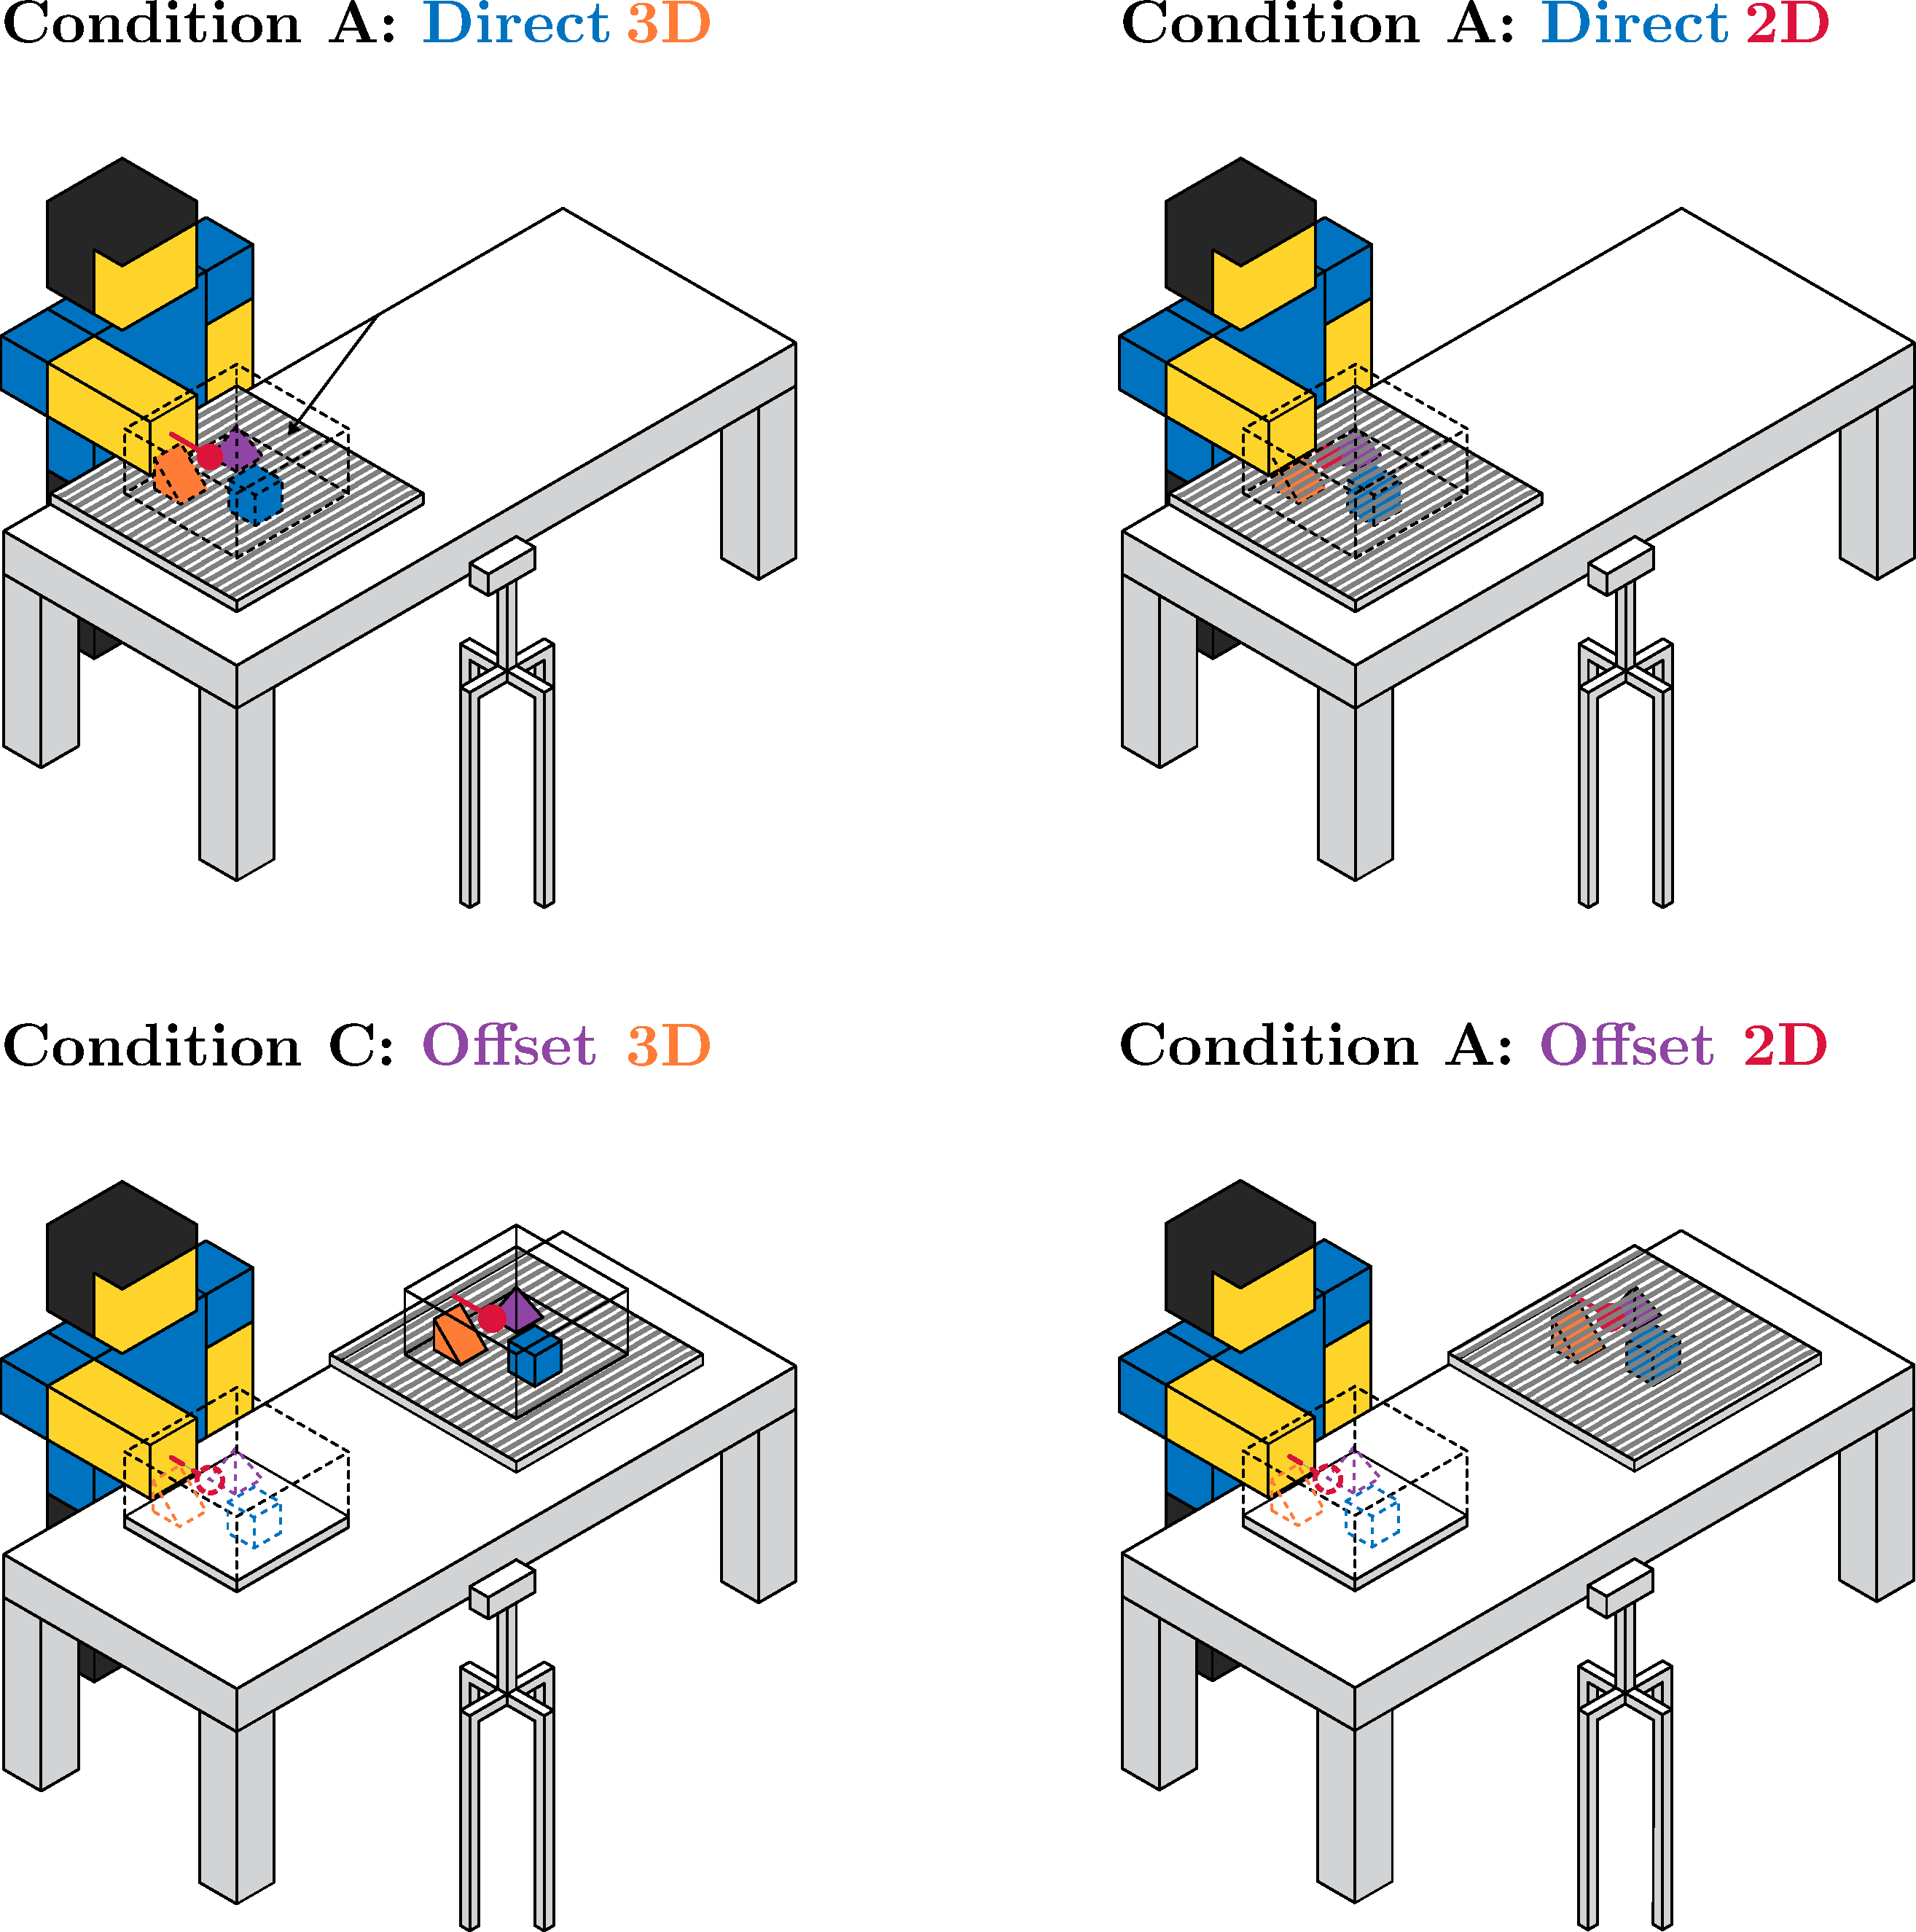
\includegraphics[width = 0.9\linewidth]{./evaluation plan/figures/user study.pdf}
\end{figureBox}
We plan to run a user study with two conditions as can be seen in \ref{fig:user-study}. In the first, condition A, we plan to have the participant interact in a virtual task with their hands directly interacting with the objects where they percieve they are. In the second, condition B, we plan to have the participant interact with the scene in a second offset interaction zone while they perceive their interactions on a separate display. This will test the ease at which a user can interact with a volumetric display via teleoperation. We will measure the time taken to complete the task and the number of errors made. We will also ask the participants to fill out a questionnaire to measure their subjective experience. We will then compare the results of the two conditions to see if there is a significant difference in the time taken to complete the task and the number of errors made. We will also compare the results of the questionnaire to see if there is a significant difference in the subjective experience of the two conditions.

\section{Novel Contributions}
Once this project is complete we expect to have made the following novel contributions:
\begin{itemize}
    \item A \textbf{volumetric display simulator} that is Multi-platform, Lightweight, Cheap, Simple, and Reproducible.
    \item A \textbf{user experiment} that compares the effectiveness of using hand tracking to interact directly with an ethereal/incorporeal volumetric display compared to a via teleoperation with a corporeal/tangible display.
\end{itemize}